\chapter{Introduction} 

\label{chap:introduction} 

%----------------------------------------------------------------------------------------
\section{Semantic Memory, Representation and Processing} 

Semantics as in linguistic context, is the connection between language forms such as orthography, syntax, and meanings including lexical and phrasal ones. The brain processes semantics in aide of semantic memory \parencite{tulvingEpisodicSemanticMemory1972}, of which the loci in human cognition system are still actively being debated. 

Semantic memory is unlike episodic memory, which is individual-specific and modality dependent. As semantic memory is associated with general world knowledge \parencite{mcraeSemanticMemory2013}, semantic memory tends to be shared across individuals within a common cultural background. Such invariance provides a window for semantic memory loci localization in the human brain. 

In \citeauthor{tulvingEpisodicSemanticMemory1972}'s view, semantic memory is conceptually dissociated, but not necessarily functionally or structurally separated from procedural and episodic memory. However, studies \parencite{vargha-khademDifferentialEffectsEarly1997} suggest the structural and functional dissociation of episodic memory and semantic memory, and that parahippocamal cortices, as a classical theoretical locus of episodic memory, are not crucial for the normal functioning of semantic memory.

\begin{table}

\centering

\begin{tabularx}{\textwidth}{@{} L *{5}{X} @{}}
\toprule
\tabhead{Reference} & \tabhead{Frontal Lobe} & \tabhead{Temporal Lobe} & \tabhead{Parietal Lobe} & \tabhead{Occipital Lobe} & \tabhead{Limbic Lobe}\\
\midrule
\cite{tsukiuraDissociableRolesBilateral2006} & IFG & CA, STG & AG & GF & PCG \\
{[}TODO More weekend{]} &  &  &  &  &  \\
\bottomrule \\
\end{tabularx}
\caption{Involvement of Cerebral Areas in Semantic Tasks}
\label{tab:distributedareastudysynthesis}
\end{table}
    

While some theorist argue for the temporal localization of semantic memory~\parencite{saumierSemanticMemory2002, martinSemanticMemoryBrain2001}, recent studies found neural correlates of semantic knowledge distributed in multiple lobes (refer to Table \ref{tab:distributedareastudysynthesis} for a resume), supporting thus the distributed hypothesis that semantic knowledge might be encoded in multiple brain areas. The cortices involved in semantic processing other than the temporal cortex, are strongly associated to perceptual, sensorial and/or affectual functions, suggesting that semantic memory depends on episodic events~\parencite{moseleyNounsVerbsObjects2014}. 

A theoretical reconciliation between these two schools is the specialization of cortical areas implicated in semantic tasks: the abstract, amodal semantic memory being grounded by concrete modal episodic memories \parencite{pecherGroundingCognitionRole2005}. 

The classical semantic memory locus could serve as the convergence zone for binding information from modality-specific cortices \parencite{damasioNeuralBasisLexical1996, damasioNeuralSystemsWord2004, simmonsSimilarityintopographyPrincipleReconciling2003}. Anatomical evidences, that the possible loci sit at convergences of multiple perceptual processing streams \parencite{binderNeurobiologySemanticMemory2011}, support this theory. \textcite{pattersonWhereYouKnow2007} further exploited \citeauthor{damasioNeuralSystemsWord2004}'s arguments by proposing the \emph{Hub-and-Spoke} model, where a semantic hub, not only acts as a pointer and a information-binder, but also constructs, refines semantic concepts and builds cross-modal similarity structures using episodic event. In parallel, \textcite{paivioMindItsEvolution2008} argued for a dual-coding system to address the problem of representing abstract concepts which do not necessarily have perceptual input: in addition to accumulated perceptual information for concrete concepts, a more meta-semantic department keeps record for all concepts. 



In this project, we restrain the discussion to lexicosemantic system, particularly we will focus on the representation and processing of word meanings in an ecological auditive experiment. 

\section{Syntagmatic and Paradigmatic Axes in Linguistics}
\label{sec:IntroSyntagandParaAxies}
\textcite{jakobsonFundamentalsLanguage1963} and \textcite{desaussureCoursLinguistiqueGenerale1969} propose that all linguistic units are arranged in two modes which are \emph{combination} and \emph{selection}, or \emph{syntagm} and \emph{paradigm}. \emph{Combination} is in \emph{presentia} as the linguistic unit (in the current context, a word / lemma / lexicon unit) is contextualized by other elements presented in a linguistic sequence. \emph{Selection} is in \emph{absentia} as it is linked to other alternative substitutions which are absent from the current context. Table \ref{tab:egsyntagparadig} gives an example of the organization in two axes.

\begin{table}
    \centering
    \begin{ThreePartTable}  
    \begin{tabularx}{\textwidth}{p{3mm}p{1mm}*{7}{L}}
     & \multicolumn{7}{c}{\tabhead{syntagmatic}} \\
     \parbox[t]{1mm}{\multirow{7}{*}{\rotatebox[origin=c]{90}{\tabhead{paradigmatic}}}} & \tikzmark{ps} & \tikzmark{ss} &  &  &  & & &  \tikzmark{se} \\
    & & The & ridiculous & girl & fell & into & the & pond. \\
    & & & \textcolor{gray}{silly} & \textcolor{gray}{person} & \textcolor{gray}{jumped} & & & \textcolor{gray}{river.} \\
    & & & \textcolor{gray}{foolish} & \textcolor{gray}{woman} & \textcolor{gray}{tripped} & & & \textcolor{gray}{lake.} \\
    & & & \textcolor{gray}{funny} & \textcolor{gray}{lady} & \textcolor{gray}{plunged} & & & \textcolor{gray}{sea.} \\
    & & & \textcolor{gray}{crazy} & \textcolor{gray}{princess} & \textcolor{gray}{walked} & & & \textcolor{gray}{ocean.} \\
    & \tikzmark{pe} & & \textcolor{gray}{klutzy} & \textcolor{gray}{child} & \textcolor{gray}{ran} & &  & \textcolor{gray}{pool.} \\
    \end{tabularx}
    \end{ThreePartTable}
    \caption[Example of Syntagmatic and Paradigmatic Axes]{An example of syntagmatic and paradigmatic axes. Gray-colored texts are in \emph{absentia}, black-colored texts are in \emph{presentia}. \emph{Syntagm} combines word sequence into a meaningful sentence, while \emph{paradigm} provides feasible substitutions of currently-present words.\label{tab:egsyntagparadig}}
    \begin{tikzpicture}[overlay, remember picture, yshift=.25\baselineskip, shorten >=.5pt, shorten <=.5pt]
        \draw [->] ([yshift=.75pt]{pic cs:ps}) -- ({pic cs:pe});
        \draw [->] ([yshift=.75pt]{pic cs:ss}) -- ({pic cs:se});
      \end{tikzpicture}
\end{table}


\citeauthor{jakobsonFundamentalsLanguage1963} further illustrated the twofold character of language via selection-deficient and contexture-deficient aphasics using data from \textcite{goldsteinLanguageLanguageDisturbances1948, headAphasiaKindredDisorders1920, hughlingsjacksonAffectionsSpeechDisease1879, goldsteinProblemMeaningWords1971, luriaWorkingBrainIntroduction1976c, crutchAbstractConcreteConcepts2004, warringtonCategorySpecificAccess1983}, bridging formal linguistic works with psycholinguistic studies.

Similarity disorder (selection-deficiency) patients are able to complete scraps of words or sentence, but are unable to uncontextualize themselves, thus unable to utter ''it rains'' unless it rains actually. The retrieval of the most precise lexicon is blocked, and the internal relation between concepts are dissolved. For those patients, an isolated word means nothing, occurrences of one same word in different contexts are homonyms, and the production of word tends to be bound by other associative words (for example, \emph{knife} are referred to as \emph{pencil-sharpener}, \emph{bread-knife} and \emph{knife-and-fork}) or metonymies (\emph{fork} for \emph{knife}, \emph{eat} for \emph{toaster}), or replaced by the most general terms such as \emph{chose} and \emph{machin} in French. The utterances are highly dominated by spatial, temporal and usage proximities, which are not necessarily parallel to similarity. They also lose the ability to switch register and stay in their idiolect reality. As remarked by \citeauthor{jakobsonFundamentalsLanguage1963}, for such an aphasic whose substitutional capacity has been disabled and contextual capacity intact, the emissive and receptive linguistic competence relies solely on contiguity. 

Contiguity disorder (contexture-deficiency) patients, on the other hand, are impaired to propositionize, inflect and desolve compound words such as \emph{thanksgiving} into \emph{thanks} and \emph{giving}. They produce agrammatical sentences as a chaotic word heap. The approximative identifications of a presented concept are quasimetaphoric (such as \emph{spyglass} are produced for \emph{microscope}, \emph{fire} for \emph{gaslight}), without any deliberate transfer of meaning as it is in the case of poetry and rhetorics. 

%----------------------------------------------------------------------------------------

\section{Computational Semantic Representation Modeling}

Natural language processing and understanding in general artificial intelligence has partially branched away from cognitive computational linguistic works. While language representation models like BERT~\parencite{devlinBERTPretrainingDeep2018} are fine-tuned to natural language processing benchmark tasks, they do not necessarily approach human language processing. We restrain computational semantic modeling to the models attempting to replicate of human linguistic dynamics. 

Semantic representation models digitalize the natural language word meanings into numeric representations that can be understood and processed by neural networks and computer systems. There are two schools of modeling: symbolic and distributional.

\subsection{Symbolic Relational Semantic Models}

\label{subsection:symbolicembedding}
Classical semantic models assumes the meanings can be considered as an indexable binary feature array \parencite{smithSemanticMemoryPsychological1974} or interconnected nodes in a large semantic graph-like ontological network \parencite{collinsRetrievalTimeSemantic1969}. In such structures, the binary features and nodes in the ontologies each represents a semantic entity (\emph{symbol}), to which we associate properties or values. Depending on the implementation, such symbolic structures are usually abstracted or independent from episodic, perceptual experiences. They are able to account for abstract taxonomical conceptual comparisons. Therefore, they model mainly paradigmatic similarities. 

Modern implementation of such models still rely largely on human manual coding. WordNet-alike knowledge bases \parencite{millerWordNetLexicalDatabase1995, millerWordNetElectronicLexical1998, sagotBuildingFreeFrench2008, pradetWonefImprovedExpanded2014} are examples of symbolic semantic networks which encodes inter-word semantic relations. In this class of models, lexicon units are regrouped into \emph{synsets}, forming synonymy sets, each representing one different meaning of the unit. Synsets are interconnected with relations such as \emph{antonymy, hyponymy, hypernymy, meronymy, toponymy}\dots

\subsection{Statistical Distributed Representations}

\label{subsection:statisticalembedding}

\textcite{harrisDistributionalStructure1954}'s distributional hypothesis argues that ``linguistics items with similar distributions have similar meanings.'' Most statistical models based on this theoretical foundation could be classified into latent semantic inference models \parencite{deerwesterUnitedStatesPatent1989, penningtonGloveGlobalVectors2014} and hyperspace analogue to language models \parencite{burgessHyperspaceAnalogueLanguage1995, mikolovEfficientEstimationWord2013, levyDependencyBasedWordEmbeddings2014}. As they make heavy use of contextual information, the syntagmatic information are also present those classes of models.

Such representation models use high dimensional vectors to encode semantic entities. The 2D matrix representation of the model, where the rows are entries of the lexicon, columns being the vector dimensions, are referred to as \emph{semantic embeddings} or \emph{semantic spaces}. Similarity measures are derived on vector distance metrics including cosine distance, gaussian distance and Minkowski distances. Models such as \textcite{penningtonGloveGlobalVectors2014, mikolovEfficientEstimationWord2013} successfully capture semantic information from textual statistics, achieving adequate performance on similarity benchmarks. 

On the linguistic nature of statistical distributed representation (SDR) models, we observed a mixture of syntagmatic and paradigmatic information in statistical embeddings. To give an example, in an openly available GloVe~\parencite{penningtonGloveGlobalVectors2014} implementation\footnote{Wikipedia 2014 + Gigaword 5 with 6B tokens, 400k uncased vocabulary and 300 dimensions. \url{https://nlp.stanford.edu/projects/glove/}.}, the closest neighbors of the target word \emph{teacher} (a noun) are composed of synonyms (\emph{instructor, tutee}) and associates (\emph{classroom, teaching, school, student, aunt\dots}) (Table \ref{tab:gloveneighbours}).  While the list of synonyms proposed by WordNet is \emph{instructor, teaching fellow, docent, coach}, which is purely paradigmatic.


\begin{table}
    \centering
    \begin{ThreePartTable}  
    \begin{tabularx}{\textwidth}{*{4}{L}}
    \multicolumn{2}{l}{\tabhead{Target word:}} & teacher & \\
    \toprule
    \tabhead{Neighbour} & \tabhead{Cosine Distance\tnote{1}} & \tabhead{Nature of Neighbour} & \tabhead{Semantic Relation} \\
  \toprule
classroom & 0.537 & associate & locative \\
teaching & 0.497 & associate & action \\
school & 0.484& associate & locative \\
preschool & 0.453 & associate & locative \\
student & 0.421& associate & object/agent\\
grade & 0.418 & associate & \\
college & 0.403 & associate & locative \\
instructor & 0.401 & synonym & \\

    \bottomrule
    \end{tabularx}
    \begin{tablenotes}
        \footnotesize
        \item[*] A cosine distance near 0 indicates a greater similarity.
    \end{tablenotes}  
    \end{ThreePartTable}
    \caption[Example of Syntagmatic and Paradigmatic Mixture in Statistical Semantic Models]{\emph{Teacher} are judged to be close to \emph{classroom, teaching, student}\dots. While they are frequent collocations, they are nevertheless not synonyms. \label{tab:gloveneighbours}}
\end{table}

\textcite{lapesaContrastingSyntagmaticParadigmatic2014} tested combinations of different hyper-parameters of co-occurrence-based statistical representation building algorithm. They used behavioral priming data of syntagmatic and paradigmatic word-pairs to contrast parameters' influence on two axes' performance. Figure \ref{fig:synparacontextwindow} is reproduced using the reported data from the work, confirming more systematically the two-fold mixture in SDR embeddings.

\begin{figure}
    \centering
    \makebox[\linewidth]{
    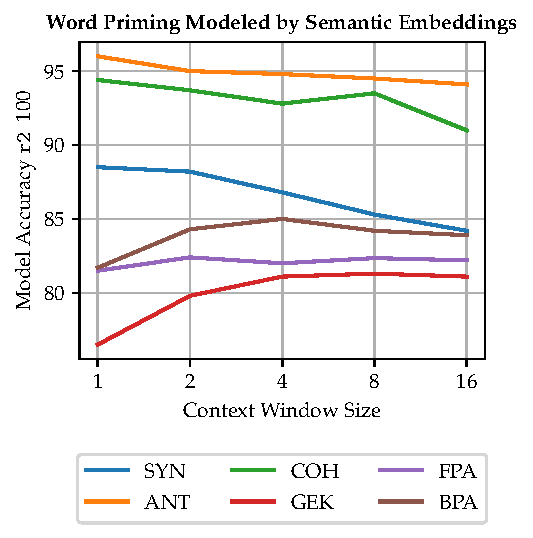
\includegraphics[scale=1]{Figures/SynParaContextWindow.pdf}
    }
    \caption[Impact of Context Window Size on Syntagmatic and Paradigmatic Information Extraction]{\textcite{lapesaContrastingSyntagmaticParadigmatic2014} tested 6 priming scheme datasets: paradigmatic datasets include synonyms \code{SYN}, antonyms \code{ANT} and cohypernyms \code{COH}, syntagmatic datasets include forward phrasal associates \code{FPA}, backward phrasal associates \code{BPA} and generalized event knowledge \code{GEK}. For each of the 6 datasets, they trained a separate GLM using differently configured semantic embeddings to predict word priming delays. Increasing context window size when training the embedding improves syntagmatic model accuracy, while penalizes paradigmatic predictions. Note that paradigmatic results are consistently better than syntagmatic ones.} 
    \label{fig:synparacontextwindow}
\end{figure}


%----------------------------------------------------------------------------------------

\section{Semantic Neural Encoding/Decoding Experiments}

The cognitive account of semantic processing includes the identification of the specific functions of various cortical areas during the semantic process. Historically, neuroscientists had to rely on semantic deficits and lesion studies. With cognitive modeling development, neuroimaging techniques enabled the examination of various model proposals without having to open the skull. 

\textcite{marrVisionComputationalInvestigation1982} proposed the three levels of modeling in: \emph{computation, algorithm} and \emph{implementation}. On operating on the computational level, cognitive modelers either try to replicate the temporal-spatial dynamics of cerebral activities, thus \emph{encodes} neural signals, and/or use measured signals to recover external stimuli, thus \emph{decodes} brain activity. 

Given the temporal and spatial resolution constraints of neuroimaging techniques among electroencephalography (EEG), magnetoencephalography (MEG), functional magnetic resonance imaging (fMRI), positron emission tomography (PET), fMRI and PET gained enormous popularity in the semantic localization studies while MEG for spatial-precise temporal dynamic studies~\parencite{molloOscillatoryDynamicsSupporting2017}. fMRI gives a much better spatial resolution than EEG (up to millimeters), but it is generally poor in temporal resolution. Classic semantic stimuli units are presented at sub-second level (hundreds of milliseconds) but the usual imaging frequency is at second level, and the measured blood-oxygen-level dependent (BOLD) signal approximates a temporal convolution of real neuron activation and hemodynamic function over 4 to 7 seconds.

Encoding and decoding experiments heavily rely on computational semantic representation models, especially distributed representations. \textcite{mitchellPredictingHumanBrain2008} was the first work to use contextual co-occurrence vectors (one variate of SDR) to encode semantic processing activities for concrete nouns. The predictive model showed significant generalization power, indicating a strong association between semantic embeddings and the brain activity, and the feasibility of encoding fMRI recorded semantic brain activity.

\subsection{Multi-Network Participation in Semantic Processing}
\label{subsec:multinetworkParticipation}
A large amount of literatures with encoding and decoding experiments report results in favor of distributed semantic processing in the human brain. 

\textcite{mitchellPredictingHumanBrain2008}'s concrete noun encoding experiments reported the most accurately predicted voxels to be located in (pre)frontal, parieto-temporal regions. \textcite{pereiraUniversalDecoderLinguistic2018} used fMRI signals to decode lexical and phrasal semantic stimuli presented in isolation. Among the 5000 most informative voxels found for each subject, functional networks in human brain other than the linguistic one take also a significant portion consistently across subjects. 

In addition to experiments conducted with isolated semantic stimuli, works such as \textcite{todorovicAnalysesIRMfLors2018, verdierEncodageActiviteNeuronale2018} [TODO, add more refs] experimented with ecological stimuli. They found consistent encoding / decoding performance with non-classically-linguistic cortical area voxels.

Multiple theories exist to account for the contribution of other cortical areas in semantic processing.   

\subsubsection{Evidences for Feature-Based Distribution}
\label{subsec: featurebaseddistribution}
Feature-based distributional models argue that various cortices are recruited to encode modality-specific information~\parencite{chaoAttributebasedNeuralSubstrates1999, haukSomatotopicRepresentationAction2004, goldbergPerceptualKnowledgeRetrieval2006}. The parallel activations of these areas participate in the completion of semantic retrieval and representation~\parencite{pattersonWhereYouKnow2007}. Experiments \parencite{borghesaniWordMeaningVentral2016} successfully decode perceptual information (size, [TODO] \dots) associated with isolated words using only textual stimuli. \textcite{huthNaturalSpeechReveals2016} proposed a semantic cortical mapping organized by PCA-generated semantic axes including perceptual properties (e.g. visual, tactical, emotional, locational) along with semantic domains(e.g. tools, animals, living animates). \textcite{rowtulaDeepAutoencoderNearPerfect2018} mixed textual semantic embeddings with image-based (visual) semantic embeddings to encode \textcite{pereiraUniversalDecoderLinguistic2018}'s data. The multimodal model, compared to purely textual ones, gave much better results in fMRI encoding.

\subsubsection{Evidences for Semantic-Domain-Based Distribution}

Domain-specific distributional models \parencite{damasioNeuralBasisLexical1996, damasioNeuralSystemsWord2004, mahonWhatDrivesOrganization2011} argue for a cortical map in function of semantic categories (\emph{domains}, such as living animate, vegetables, tools). The argument is mainly supported by category-specific pathology observations: cortical connectivity are locally tuned for different semantic topics' operational processing. 

\textcite{huthContinuousSemanticSpace2012} used WordNet-based noun and verb hierarchical structures to correlate neural responses in different cortical area with word categories (\emph{semantic domain}, e.g. \emph{athlete, communicate}). Analysis showed that voxels in [TODO replace labels by understandable names: IFSFP, FO, AC, FFA, PPA, COS, ITS, V1-V7, OFA, LO, IPS, RSC, MPC \dots ] responded to different domain-specific words. The semantic axes of \textcite{huthNaturalSpeechReveals2016} mentioned in Section \ref{subsec: featurebaseddistribution} include also domain-specific ones.

Importantly, semantic features and domains are not necessarily two dissociated principles of semantic organization. For example, domain traits can also imply \emph{feature} information (domestic animals imply the size of the concept in question shall normally not surpass that of an adult human.) [TODO: better example]

\subsubsection{Evidences for Semantic Control Networks}
\emph{Controlled Semantic Cognition} \parencite{ralphNeuralComputationalBases2017} system argues for an operational rather than representational account. CSC argues for a semantic hub\parencite{pattersonWhereYouKnow2007}, and it considers the neural correlates in non-hub areas as the interaction with semantic representation system and the computation of semantic entities and non-linguistic decision making~\parencite{fusterUpperProcessingStages2004}. Semantic computation, such as combination and selection, is modulated by linguistic and task contexts. Since language is also a social tool, goal, action and decision making is also implicated in semantic processing. These functions recruit the cortices revealed by semantic encoding/decoding experiments. 
%----------------------------------------------------------------------------------------

\section{Outline}

This master's project attempts to examine different cortical regions' participation in the two semantic processing axes,which we name as \similarity and \association. We attribute each axis, or organisational principle, with a fine-tuned semantic representation model, configured with our assumptions and hypothetical properties on these axes. 
Through an fMRI encoding experiment using lexical semantic models in an ecological setting, we infer each region's functional properties based on the locally preferred organisational principle.

In chapter \ref{chap:hypotheses}, assumptions on \similarity and \association axes and semantic distributional representation structures are presented and discussed along with the semantic memory localization hypotheses. In chapter \ref{chap:methods}, we will present our methods on building semantic representations, preliminary assumption validations, fMRI encoding settings and result interpretation. Then the obtained results are presented in chapter \ref{chap:results}. We will present further ad-hoc analyses and possible implications of our results in chapter \ref{chap:discussions}.